\documentclass[12pt,a4paper,portuguese]{article}

\usepackage[brazil]{babel}
\usepackage[utf8]{inputenc}
\usepackage[T1]{fontenc}
\usepackage[margin=1.5cm]{geometry}
\usepackage{graphicx}
\usepackage{float}
\usepackage{tikz}
\usetikzlibrary{arrows.meta,decorations.markings,decorations.pathmorphing}
\usepackage{amsmath}
\usepackage{amssymb}
\usepackage{mathtools}

\usepackage{hyperref}
\hypersetup{
	hidelinks,
	linkcolor = blue
} % Changes the link color to black and hides the hideous red border that usually is created

\begin{document}
    % Título
    \vspace{5mm}
    \rule{0.95\textwidth}{1pt}
    \vspace{3mm}
    \begin{center}
        \textbf{\huge Bad Ice Cream} \\
        \Large Projeto Final \\
        \large SCC0204 Programação Orientada a Objetos
    
        \vspace{8mm}
        \begin{tabular}{rcl}
            Amanda Pereira da Silva &-- &12680861 \\
            Cody Stefano Barham Setti &-- &4856322 \\
            Ian de Holanda Cavalcanti Bezerra &-- &13835412
        \end{tabular}

    \vspace{8mm}
    02 de Maio de 2025
    \end{center}

    \vspace{1mm}
    \rule{0.95\textwidth}{1pt}
    \vspace{0.5cm}

    % Corpo do texto
    \section{Orientações}
    \subsection{Inicialização do Jogo}
        Para jogar o \emph{video game} que desenvolvemos, abra no NetBeans o diretório \verb|Jogo-BadIceCream/|. Este é o nome dado ao nosso projeto NetBeans, em referência ao jogo \emph{Bad Ice Cream}, da desenvolvedora de jogos britânica \emph{Nitrome}, o qual serviu de base para quase que toda a lógica de jogo (como também os recursos visuais) de nosso projeto, uma espécie de `versão rudimentar' de \emph{Bad Ice Cream}.

    \subsubsection{Inicialização do Jogo em Fase Específica}
        Por padrão, o jogo inicia-se na primeira fase e prossegue até a quinta, a última. Entretanto, caso queira iniciar o jogo em uma fase específica, basta que mude, no código fonte, o argumento repassado a \verb|controller.carregarFase()|, no arquivo \verb|src/Main.java|, de \verb|1| à fase desejada, que, após recompilação, o jogo iniciar-se-á de tal fase.
        
        Por exemplo, \verb|controller.carregarFase(3)|, inicia o jogo na terceira fase.

    \subsection{Condições de Parada (Sucesso e Falha)}
        O objetivo é o mesmo em todas as fases: coletar todas as frutas presentes nela sem contactar os vilões (e, no caso do `vilão 2', as bolas de fogo que emite também). Ademais, na última fase, há `pisos de fogo', que só podem ser atravessados verticalmente, e nos quais não é permitido repousar.
        
        Você possui um número ilimitado de tentativas para completar cada fase. Quando falhar, precione a tecla \verb|R| para tentar novamente a fase atual.
        
    \subsection{Controles do Protagonista}
        Utilize as teclas direcionais para movimentar o protagonista do jogo. Alternativamente, você pode `teletransportá-lo' a uma posição desejada precionando com o indicador do mouse sobre tal posição.
        
    \subsection{Inserção de Vilões Adicionais na Fase Atual}
        No diretório \verb|DragAndDrop/| há arquivos \verb|.zip|, cada um contendo um dos três vilões presentes no jogo. Para adicionar um novo vilão à fase atual do jogo, para além dos seus vilões padrões, arraste com o mouse o arquivo \verb|.zip| do vilão de interesse à posição no jogo na qual deseja inseri-lo.
        
    \subsection{Salvar e Carregar Partida}
        Para salvar seu progresso no jogo, precione a tecla \verb|F5|. Para carregar a informação salvada, precione a tecla \verb|F9|. Vale salientar que eventuais vilões adicionados à fase também serão salvos.
    \section{Diagrama de Classes UML}
    \begin{figure}[H]
        \centering
        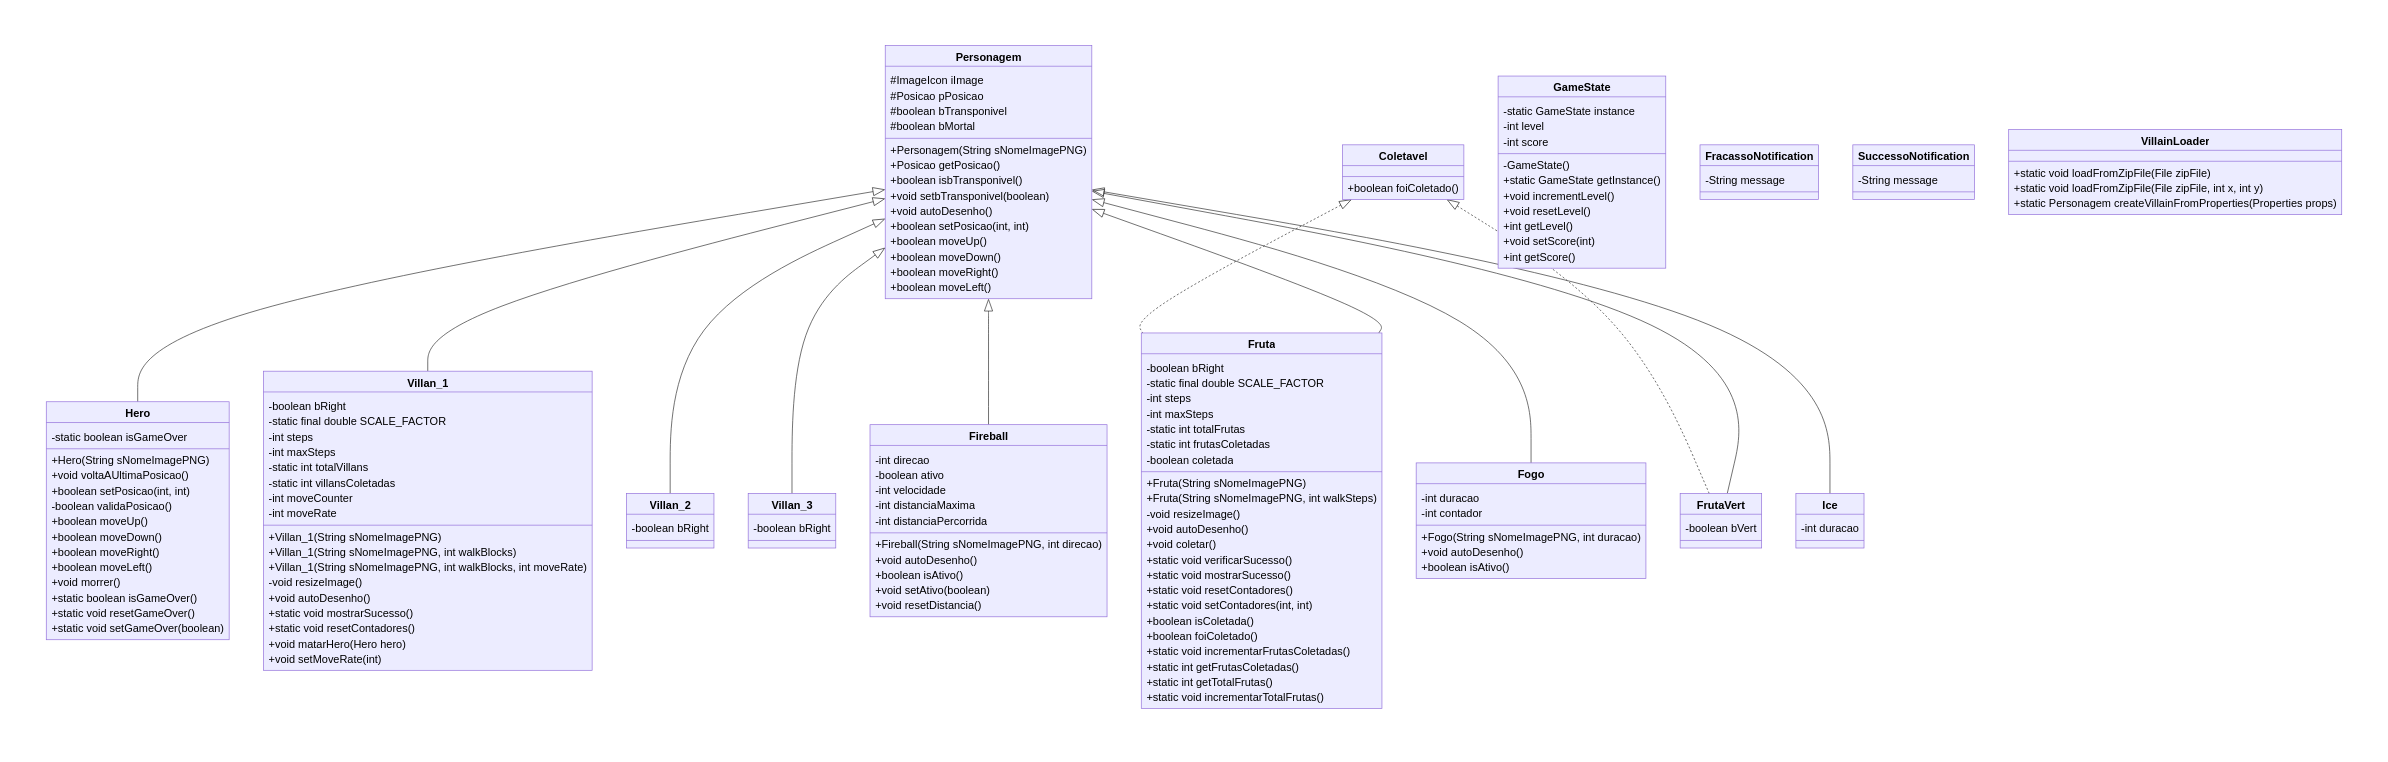
\includegraphics[width=1\textwidth]{class-diagram.png}
        \caption{Diagrama UML -- Projeto Bad Ice Cream}
        \label{fig:class-diagram}
    \end{figure}
\end{document}
